% This file is iccc.tex.  It contains the formatting instructions for and acts as a template for submissions to ICCC.  It borrows liberally from the AAAI and IJCAI formats and instructions.  It uses the files iccc.sty, iccc.bst and iccc.bib, the first two of which also borrow liberally from the same sources. The format has been updated for the ICCC2022 to include a new, mandatory section to be included in camera-ready manuscripts.


\documentclass[letterpaper]{article}
\usepackage{iccc}


\usepackage{times}
\usepackage{helvet}
\usepackage{courier}
\usepackage{amsmath}
\usepackage{musicography}
\usepackage{graphicx}
\usepackage[font=small,skip=4pt]{caption}
\usepackage{arydshln}

\pdfinfo{
/Title (Formatting Instructions for Authors)
/Subject (Proceedings of ICCC)
/Author (ICCC)}
% The file iccc.sty is the style file for ICCC proceedings.
%
\title{Converting DNA to Music: Sonifying Structure, Splicing, and Translation}
\author{Anonymous (as requested on submission instructions)\\
Anonymous Department\\
Anonymous College\\
City, State Zip Country\\
Email\\
}
\setcounter{secnumdepth}{0}

\begin{document} 
\maketitle
\begin{abstract}
The sonification of genetic material is a little-explored mode of unconventional computation bridging the divide between bioinformatics, computer science, and music, allowing scientists and non-scientists alike to perceptualize genomics in a novel and illuminating manner. This paper presents BioMus, an original model converting DNA to music as MIDI piano chords. Gene sequences are sourced from Ensembl, a genome database of the European Bioinformatics Institute, and are parsed into their constituent exons and and introns. Exons are further parsed into their 5’ and 3’ untranslated regions (UTRs) and CDS (CoDing Sequence, i.e. the protein-coding region). Then, each codon in the CDS is mapped to a major or augmented triad based on the amino acid it encodes, and individual nucleotides in introns and UTRs are respectively mapped to diminished triads and dyads outlining a minor triad. Rhythmic alterations indicate spliced CDS codons. To further emphasize protein-coding regions, all CDS chords are played at a higher volume. By mapping nucleotides and codons to musical chords, BioMus introduces a novel and straightforward means of conceptualizing both the structure of a gene and the processes of biological splicing and translation that is accessible to users of all scientific backgrounds.

\end{abstract}

\section{Introduction}
Bioinformaticists constantly seek new ways to computationally represent and interpret genomic data. Representation of genetic sequences is primarily visual, with tools such as SnapGene that visualize DNA sequences with the four nucleotides (adenine (A), cytosine (C), guanine (G), and thymine (T)) in colors \cite{goldstein_2023}.
Comprehending such visual methods generally requires a high degree of technical background, thus limiting the audience. BioMus presents a novel means of conceptualizing genomics aurally, rather than visually, in a straightforward manner that elucidates the structure of a gene as well as the essential biological processes of splicing and translation. By bridging the divide between bioinformatics, computer science, and music, BioMus’ sonification model makes these core concepts in genomics accessible to a wide-ranging audience. It particularly offers visually impaired users a newly illuminating perspective on genomics.

BioMus takes in a DNA sequence of a single gene and converts it to a series of MIDI piano chords. Genes consist of sequences of double-stranded DNA, which are built with pairs of complementary nucleotides (A-T and C-G). 
%The double-stranded DNA helix is shaped like a ladder, where each rung consists of two complementary nucleotides paired together. 
%The DNA helix consists of the \textit{coding strand} and the \textit{template strand}. The template strand codes for mRNA during $transcription$, where each nucleotide is converted to its complement, and thymine is replaced with the base uracil.% https://www.khanacademy.org/science/ap-biology/gene-expression-and-regulation/transcription-and-rna-processing/a/overview-of-transcription
DNA is converted to mRNA during transcription, and mRNA is converted to amino acids (the building blocks of proteins) during translation. Eukaryiotic transcription includes a stage called RNA splicing, where regions known as introns are removed, or “spliced out,” from the DNA sequence. The final “mature” mRNA consists of the remaining regions, called exons, strung together. The exons comprising mature mRNA consist of two untranslated regions, or UTRs, flanking the CoDing Sequence, or CDS, that codes for proteins. 
%The CDS is a sequence of nucleotides corresponding with the sequence of amino acids in a protein during translation. It begins with the start codon (ATG) and terminates with a stop codon (TAA, TAG, or TGA). 
The UTR preceding the CDS is the 5’ UTR, and the UTR following the CDS is the 3’ UTR \cite{clancy_2008,clancy_brown_2008}.

BioMus obtains gene sequences from Ensembl, a genome database of the European Bioinformatics Institute  \cite{birney_et_al_2004}. These sequences are parsed into their constituent exons and introns, and the exons are further parsed into their 5’ and 3’ UTRs and CDS. To convey the structure of the gene, individual nucleotides in introns and UTRs are mapped to diminished triads and dyads (two-note chords) outlining a minor triad, respectively. To convey translation, codons, rather than individual nucleotides, in the CDS are mapped to major or augmented triads based on the amino acids they code for.
%The opening and closing chords corresponding to start and stop codons in the CDS are also doubled in length as signposts of translation.
%To further emphasize protein-coding regions, all CDS chords are also at a higher volume. 

Pre-transcription, the UTRs and the CDS may be broken over multiple exons (i.e. they may be split by intervening introns). In the CDS, this means that individual codons may be broken across splice sites: the codon will begin at the end of one exon and conclude at the beginning of the next. To perceptualize spliced codons, BioMus splits the chord for such a codon into half its original duration and plays it both at the end of the exon that begins the codon and the beginning the next exon that completes the codon. 

%Figure \ref{fig:gene} shows the splicing process for a sample gene. The top sequence in Figure \ref{fig:gene} presents the pre-transcription DNA sequence, and the bottom sequence presents the result of splicing using \textit{complementary DNA}, or cDNA. A cDNA sequence is complementary to its source mRNA sequence;
% and contains thymine rather than uracil
%it is identical to the noncoding DNA strand without introns. Biologists synthesize cDNA from mRNA to work with the sequence more conveniently.

%\begin{figure}[h!]
%\centering
%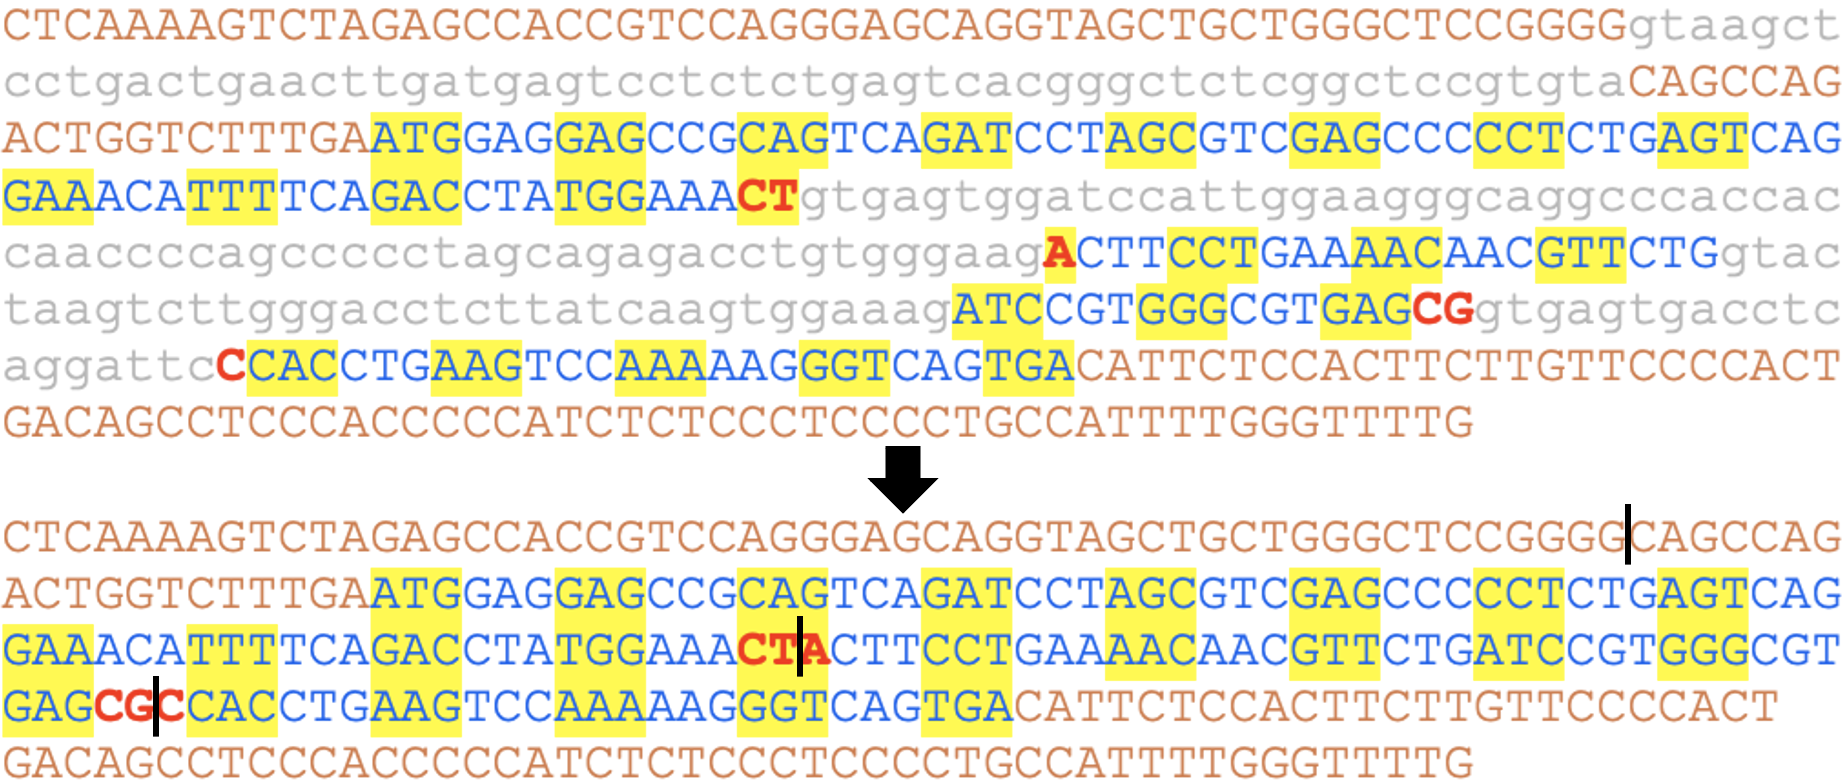
\includegraphics[width=0.48\textwidth]{images/gene.png}
 % \caption{DNA Splicing Example}\label{fig:gene}
%  \vspace{-3mm}
%\end{figure}



%In Figure \ref{fig:gene}, exons are in color, while introns are gray. The UTRs are orange, and the CDS is blue or red. Red nucleobases in the CDS indicate codons that are broken across splice sites. Notice how the 5' UTR is broken across the first two two exons, and the CDS spans the final four exons. Alternating highlights in the CDS are used for visibility of codons.  After excising the introns from the gene, the result is the contiguous sequence of exons at the bottom of Figure \ref{fig:gene}. The black vertical bars indicate splice sites. To perceptualize splicing, BioMus splits the chord for a spliced codon into half its original duration and places it at each end of the splice site: the chord will both close the exon that begins the codon and open the next exon that completes the codon. 

This paper begins by examining relevant work, then discusses the process of sourcing genetic data from Ensembl and the specifics of BioMus’ sonification model. Finally, examples of the sonification model are presented.

\section{Related Work}

Sonofication of genetic material has been approached from a variety of angles. To address accessibility of genomics to a wider audience, Takahashi and Miller convert genome-encoded protein sequences to piano notes in order to produce musical patterns that still adhere to the structure of the sequences. Their scheme maps pairs of amino acids to triads, with different inversions distinguishing individual amino acids within the pairs. The duration of each triad is determined by the frequency of the corresponding codon in the CDS. Unlike BioMus, Takahashi and Miller only consider the CDS when sonifying the gene, and they do not consider spliced codons \cite{takahashi_miller_2007}. 

Plaisier et al. also seek to increase accessibility to genomics by proposing a sonification model that is both entertaining and informative. They map nucleotides to notes to transcend the monotonous appearance of traditional DNA sequence visualizations and create the excitement expected by a public audience. By using the Sonic Pi program for sonification, they crucially support real-time customization of the program, linking DNA to live programming to further enhance public engagement. BioMus’ sonification model perceptualizes a wider variety of biological structures than Plaisier et al.’s model \cite{plaisier_meagher_barker_2021}.

In another sonification model, Ingalls et al. consider the sequence alignment problem, where sequences from the same gene but different species are compared to identify overlapping regions. Their tool \textsc{ComposAlign} translates genome-wide aligned data into music by mapping alignment information onto musical features. Their approach sonifies the presence and absence of characters (nucleotides or amino acids) in the alignment such that their assignment to the corresponding sequence (i.e. species) is clear. By mapping each character to a measure-long motif, rather than a single note or chord, \textsc{ComposAlign} achieves a mapping that is modular and flexible. Sequence alignment is outside the scope of BioMus’ current scheme \cite{mci/Ingalls2009}. 

\section{Converting DNA to Music}
\subsection{Obtaining Genetic Data}
BioMus’s sonification of DNA begins with the user specifying a desired species and gene. This information is passed to Ensembl’s REST API to obtain the chromosomal coordinates of the gene’s exons from its canonical transcript, the gene’s most conserved and highly expressed transcript in Ensembl that has the longest CDS and is also represented in other major databases such as the NCBI \cite{ensembl_transcript_flags}. The exon coordinates also define the coordinates of the intervening introns. Each pair of exon and intron coordinates is passed back to the Ensembl REST API to query for the nucleotide sequences of each region, and the result is a list of alternating exons and introns. For instance, consider the abbreviated sequence obtained from Ensembl for the \textit{Homo sapiens TP53} tumor suppressor gene in Figure \ref{fig:pre_processed_seq_homo_sapiens_tp53}. Ellipses indicate omitted nucleotides for the sake of example.

\begin{figure}[h!]
\centering
\vspace{-3mm}
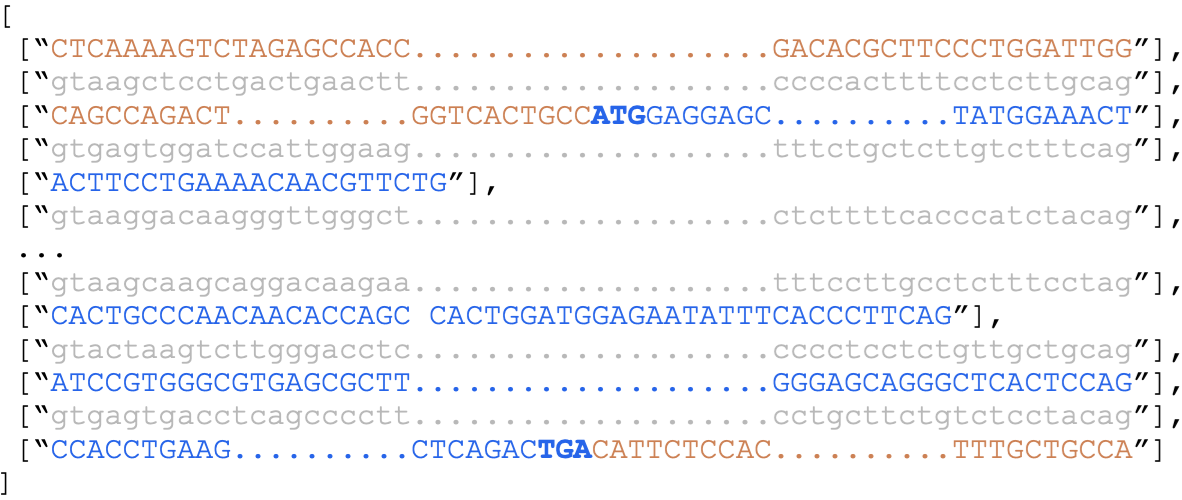
\includegraphics[width=0.48\textwidth]{images/pre_processed_seq_homo_sapiens_tp53_ABBREV}
  \caption{\textit{Homo sapiens, TP53}, Gene}\label{fig:pre_processed_seq_homo_sapiens_tp53}
  \vspace{-6mm}
\end{figure}

Exons are in color, while introns are in grey. Within the exons, orange indicates UTRs and blue indicates the CDS. Note that the CDS begins with the bolded start codon ATG and ends with the bolded stop codon TGA.

Now, the goal is to extract the 5’ UTR from the list. In order to ensure the correct start of the CDS, it is necessary to verify the 5’ UTR with Ensembl, since the 5' UTR may include multiple ATG start codons that do not signal the start of the CDS. This is not necessary for the 3’ UTR, since once we know we are in the CDS, the first stop codon will always signal the end of the CDS and the beginning of the 3’ UTR. We verify the 5’ UTR by querying the Ensembl REST API for the cDNA sequence of the canonical transcript. A cDNA sequence is complementary to its source mRNA sequence; it is identical to the original DNA without introns. Biologists synthesize cDNA from mRNA to work with the sequence more conveniently \cite{ensembl_glossary}. By requesting Ensembl to ``mask" the UTRs of the cDNA sequence by representing them in lowercase, we can successfully isolate the 5’ UTR and extract it from the list. As seen in Figure \ref{fig:post_processed_seq_homo_sapiens_tp53}, we end up with a list of the 5’ UTR regions (top), and a list of the CDS regions, introns, and the 3’ UTR (bottom).

\begin{figure}[h!]
\centering
\vspace{-3mm}
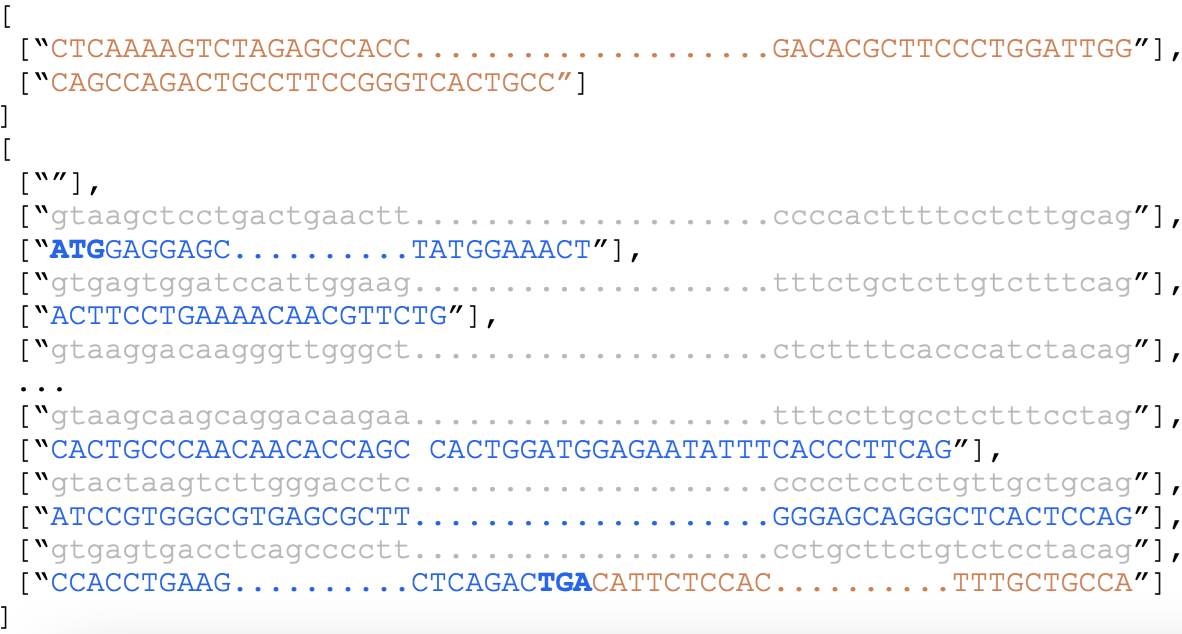
\includegraphics[width=0.48\textwidth]{images/post_processed_seq_homo_sapiens_tp53_ABBREV}
  \caption{\textit{Homo sapiens}, TP53 Gene}\label{fig:post_processed_seq_homo_sapiens_tp53}
  \vspace{-3mm}
\end{figure}

We now have all the tools necessary to translate the genetic data into music.

\subsection{Conversion to MIDI}

MIDI conversion begins by using the MIDIUtil Python library to create a MIDI track with the tempo set to \musQuarter\; = 200 BPM. Then, we begin mapping nucleotides and codons to chords within the octave C4-B4. This means that all chords built on the notes C through E will be in root position, and the remainder will be in inversion.

Sonification of the gene begins with the 5’ UTR, and the initial key is set to C minor. No key changes occur in UTRs or introns; the key is exclusively changed in the CDS and is determined by the codon. Thus, before the CDS begins, all introns and the 5’ UTR remain in the initial key of C. After the CDS begins, the key of an intron is determined by the final codon in the preceding exon (whether or not that codon is broken across the splice site). The stop codon terminating the CDS then determines the key of all subsequent introns as well as the 3’ UTR.

%To convey the structure of the gene, individual nucleobases in introns and UTRs are mapped to diminished triads and dyads (two-note chords) outlining a minor triad, respectively. To convey translation, codons rather than individual nucleobases in the CDS are mapped to major or augmented triads based on the amino acids they code for. 

Individual nucleotides in the 5’ and 3’ UTRs are mapped to dyads outlining a minor triad. BioMus maps nucleotides to notes relative to the local musical key as in Table \ref{table:nucleotides}.

\begin{table}[h!]
\centering
\vspace{-2mm}
\begin{tabular}{|l|l|}
\hline
A   & Tonic    \\ \hline
C, T & Mediant  \\ \hline
G   & Dominant \\ \hline
\end{tabular}
\caption{DNA Nucleotide Mappings}
\vspace{-3mm}
\label{table:nucleotides}
\end{table}

The dyad for each nucleotide is constructed with its base pair using the mapping in Table \ref{table:nucleotides}. For instance, if the key is C minor and we encounter the nucleotide A or T, then the dyad will consist of the notes C (tonic) and E\musFlat\; (mediant). Similarly, if we encounter the nucleotide C or G, then the dyad is E\musFlat \; and G (dominant). Together, they outline a C minor triad. All UTR dyads have quarter note durations.

Individual nucleotides in introns are mapped to diminished triads. Initially, a dyad is constructed with the mapping in Table \ref{table:nucleotides}. The dominant scale degree is then lowered a half step to form a diminished, rather than a perfect, fifth from the tonic, and finally, the diminished seventh scale degree is added to each dyad. For instance, if the key is C minor and we encounter the nucleotide C or G, then the triad will consist of the notes C (tonic), E\musFlat\; (mediant), and B\musDoubleFlat\; (diminished seventh). Similarly, if we encounter the nucleotide A or T, then the triad will consist of the notes E\musFlat, G\musFlat (dominant), and B\musDoubleFlat. We use the term “diminished triad” loosely, since technically only the latter chord has the two stacked minor thirds that formally define it as a diminished triad. However, both chords outline a diminished seventh chord and have similar enough sonorities that we dub them both diminished triads as a way of distinguishing them from major, minor, or augmented triads. Lastly, like UTRs, all intron triads have quarter note durations.

When the CDS begins, we map codons, rather than individual nucleotides, to chords. The first codon in the CDS is always ATG, the start codon, which is mapped to a C major triad and is given a half note, rather than a quarter note, duration as a signpost of the beginning of translation. Subsequent chords return to quarter notes. To further emphasize we are in a protein-coding region, the volume is doubled throughout the CDS.

To convey splicing, we also consider the scenario where a codon in the CDS is broken across splice sites (i.e. the codon is split between two exons by an intervening intron). When an incomplete codon is encountered at the end of an exon in the CDS, the subsequent exon is referenced for the remainder of the codon. The spliced codon is then represented with an eighth note triad rather than a quarter note, and the same eighth note triad is repeated at the beginning of the next exon to indicate that the remainder of the codon is found there. This is detailed in Figure \ref{fig:splice_site_example}, where exons are in color, introns are gray, and highlights elucidate codons. 

\begin{figure}[h!]
\centering
\vspace{-3mm}
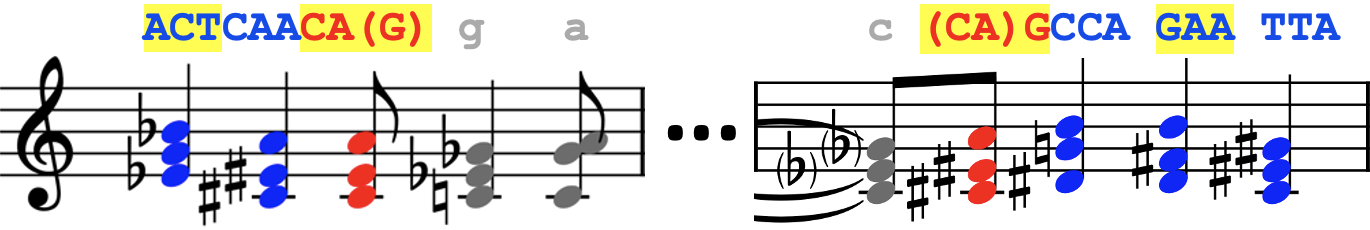
\includegraphics[width=0.38\textwidth]{images/splice_site_example}
  \caption{Spliced Codon Example}
  \label{fig:splice_site_example}
  \vspace{-3mm}
\end{figure}

The spliced codon CAG is red, with CA in the first exon and G in the second. Note how the same A augmented eighth note triad appears at both splice sites, both closing the first exon and opening the second.

Thus far, we have demonstrated a novel means to conceptualize the structure of a gene and the splicing process by differentiating between UTRs, introns, the CDS, and spliced codons. We now want to map codons in the CDS to chords in order to convey translation. To do so, we consider the amino acids the codons specify. To distinguish between amino acids, we seek an injective mapping between amino acids and musical keys. We do this by first solely considering the set of essential and nonessential amino acids (with which we can create a bijective mapping with the set of possible keys), and then separately considering the set of conditionally essential amino acids (with which we can create an injective mapping with the set of possible keys) \cite{bridges_2021}.

Figures \ref{table:essential} and \ref{table:nonessential} explicate BioMus’ bijective mapping between the set of essential and nonessential amino acids and the set of possible keys. The codons for each amino acid are listed in the left column, and BioMus maps each to a major triad in the corresponding key in the right column.

\vspace{-2mm}
\begin{table}[h!]
\centering
\begin{tabular}{|l|l|l|}
\hline
ATG & \begin{tabular}[c]{@{}l@{}}Methionine/\\Start Codon\end{tabular} & C                         \\ \hline
ATT, ATC, ATA & Isoleucine                        &  \\ \cdashline{1-2}
\begin{tabular}[c]{@{}l@{}}TTA, TTG, CTT, CTC, \\CTA, CTG\end{tabular}  & Leucine                       & C\musSharp \\ \hline
AAA, AAG &  Lysine                      & D                         \\ \hline
ACT, ACC, ACA, ACG & Threonine                       & E\musFlat  \\ \hline
TTT, TTC & Phenylalanine                       & E                         \\ \hline
TGG & Tryptophan             & F                         \\ \hline

CAT, CAC & Histidine                       & F\musSharp                         \\ \hline
GTT, GTC, GTA, GTG &  Valine                      & G  \\ \hline
\end{tabular}
\caption{Essential Amino Acids}
\label{table:essential}
\end{table}


\begin{table}[h!]
\centering
\vspace{-6mm}
\begin{tabular}{|l|l|l|}
\hline
AAT, AAC & Asparagine & A\musFlat                        \\ \hline
GAT, GAC & Aspartate  & A \\ \hline
GCT, GCC, GCA, GCG & Alanine    & B\musFlat                        \\ \hline
GAA, GAG & Glutamate    & B                        \\ \hline
\end{tabular}
\caption{Nonessential Amino Acids}
\label{table:nonessential}
\end{table}
\vspace{-2mm}

In order to achieve the bijective mapping, we simplify the alphabet of amino acids by grouping isuleucine and leucine together, since they are the most similar amino acids by Grantham's distance, a measure of evolutionary distance integrating composition, polarity and molecular volume \cite{grantham_1974}. 

Next, we consider the set of conditionally essential amino acids. Table \ref{table:conditionally_essential} explicates BioMus' injective mapping between this set and the set of possible keys. Note that the mapping is also bijective between the set of conditionally essential amino acids and the set of natural keys. Now, BioMus maps codons to augmented triads, rather than major triads, in the key in the right column to avoid overlap with the essential and nonessential amino acids.

\begin{table}[h!]
\vspace{-2mm}
\centering
\begin{tabular}{|l|l|l|}
\hline
TAT, TAC & Tyrosine                & C \\ \hline
TGT, TGC & Cysteine                & D \\ \hline
\begin{tabular}[c]{@{}l@{}}TCC, TCT, TCA, TCG, \\ AGT,  AGC\end{tabular}  & Serine                  & E \\ \hline
\begin{tabular}[c]{@{}l@{}}AGA, AGG, CGT, CGC, \\ CGA, CGG\end{tabular}  & Arginine                & F \\ \hline
CCT,  CCC, CCA, CCG & Proline                 & G \\ \hline
CAA, CAG  & \begin{tabular}[c]{@{}l@{}}Glutamine\end{tabular}  & A \\ \hline
GGT, GGC, GGA, GGG & Glycine                 & B \\ \hline
\end{tabular}
\caption{Conditionally Essential Amino Acids}
\label{table:conditionally_essential}
\vspace{-2mm}
\end{table}

Finally, we consider the stop codons, which solely serve to terminate the CDS. They are mapped to minor triads in the keys in Table  \ref{table:stop_codons}. Each stop codon chord is given a half note duration and the volume is halved to signify the end of the protein-coding region. The dyads in the 3’ UTR constituting the remainder of the gene return to quarter notes and are in whatever minor key is dictated by the stop codon in Table  \ref{table:stop_codons}.

\begin{table}[h!]
\centering
\begin{tabular}{|l|l|}
\hline
UAA & C \\ \hline
UAG & E \\ \hline
UGA & G \\ \hline
\end{tabular}
\caption{Stop Codons}
\label{table:stop_codons}
\vspace{-5mm}
\end{table}

\section{Sample Music}

Figures \ref{fig:danio_rerio_start_translation} and \ref{fig:danio_rerio_end_translation} demonstrate the sonification of key sections in the $tp53$ tumor suppressor gene of the zebrafish \textit{Danio rerio}. The DNA sequence is shown above BioMus’ sonification of each nucleotide or codon. Orange indicates UTRs, gray indicates introns, and blue indicates the CDS. Red indicates CDS codons that are broken across splice sites. Alternating codons in the CDS are highlighted for visibility

Figure \ref{fig:danio_rerio_start_translation} begins with the fragment of the 5' UTR concluding the gene's first exon. 

\begin{figure}[h!]
\centering
\vspace{-2mm}
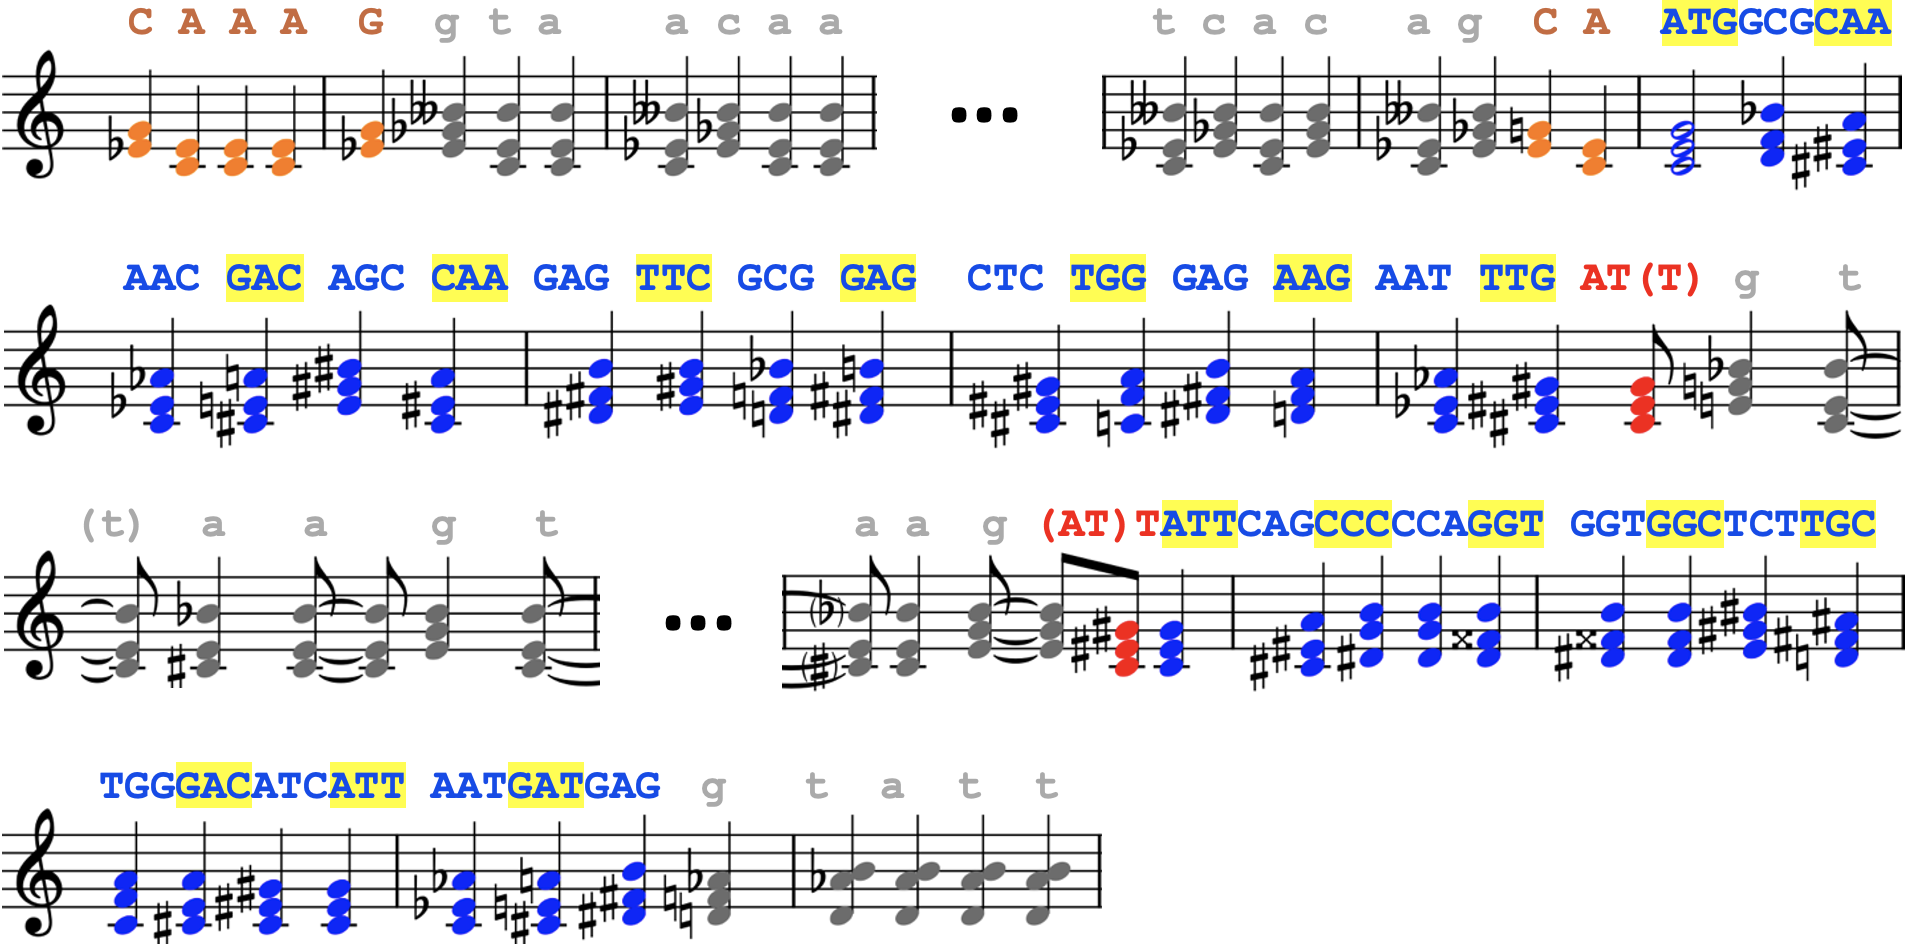
\includegraphics[width=0.48\textwidth]{images/danio_rerio_start_translation}
  \caption{\textit{Danio rerio} TP53 Gene, Beginning of CDS}
  \label{fig:danio_rerio_start_translation}
  \vspace{-3mm}
\end{figure}

Note that the opening key is C minor. The nucleotides  A and T map to the dyad C-E\musFlat \;(tonic-mediant), and the nucleotides C and G map to the dyad E\musFlat-G (mediant-dominant). We then enter the gray region of the first intron, where diminished triads outline the C diminished seventh chord (notice how the perfect fifth G above the tonic becomes the diminished fifth G\musFlat, and each triad includes the addition of the diminished seventh B\musDoubleFlat).


The second exon begins with the last two nucleotides of the 5’ UTR, which again outlines the C minor triad, before beginning the CDS with the start codon ATG, which maps to a C major triad as in Table \ref{table:essential}. Note that ATG maps to a half, rather than quarter, note to signify the start of the protein-coding region. From here, each CDS codon maps to a major or augmented triad based on Tables  \ref{table:essential}-\ref{table:conditionally_essential}. For instance, GCG codes for the nonessential amino acid alanine, which maps to a B\musFlat\; major triad as in Table \ref{table:nonessential}, while CAA codes for the conditionally essential amino acid glutamine, which maps to an A augmented triad as in Table \ref{table:conditionally_essential}.

Then, notice how ATT, which codes for the essential amino acid isoleucine and maps to the red C\musSharp\; major triad as in Table \ref{table:essential}, is broken across the splice sites between the second and third exons. The intervening intron assumes the key dictated by this final (albeit incomplete) codon, and thus outlines a C\musSharp \; diminished seventh chord. The third exon then begins with the other ``half" (i.e.  remaining eighth note) of the C\musSharp\; major triad of the spliced ATT codon. This exon concludes with the complete codon GAG, which also codes for glutamine and maps to an A augmented triad as in Table \ref{table:conditionally_essential}. The following intron assumes the same key of A, and outlines an A \; diminished seventh chord. Notably, if played, the volume in the CDS would be doubled.

Figure \ref{fig:danio_rerio_end_translation} shows part of the exon with the end of the CDS. 

\begin{figure}[h!]
\centering
\vspace{-4mm}
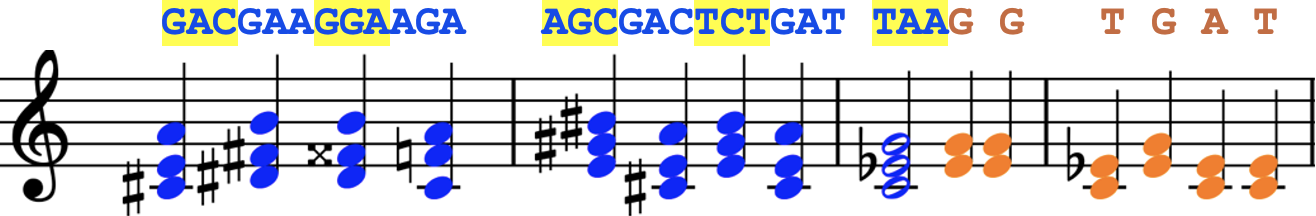
\includegraphics[width=0.48\textwidth]{images/danio_rerio_end_translation}
  \caption{\textit{Danio rerio} TP53 Gene, End of CDS}
  \label{fig:danio_rerio_end_translation}
  \vspace{-4mm}
\end{figure}

The CDS terminates with the stop codon TAA, which maps to a C minor triad as in Table \ref{table:stop_codons}. Note that TAA maps to a half note, rather than a quarter note, to signify the end of the protein-coding region. After this, we immediately enter the 3’ UTR, which assumes the key of the stop codon and thus produces dyads outlining a C minor triad.

\section{Conclusion}
BioMus serves as a bridge between bioinformatics, computer science, and music by giving scientists and non-scientists alike a novel, creative means to aurally conceptualize the structure of a gene and the biological processes of splicing and translation. Genetic structure and splice sites are illuminated by mapping individual nucleotides in UTRs and introns to diminished chords and dyads outlining a minor triad, respectively, and breaking chords across splice sites just as their corresponding codons are. Translation is conveyed by mapping CDS codons to major and augmented chords based on their encoded amino acids. The chosen injective mapping between codons and musical keys allows the listener to distinguish between essential, nonessential, and conditionally essential amino acids. BioMus’ straightforward sonification model allows users to conceptualize fundamental ideas in genomics whether or not they are career scientists, and opens to the door for visually impaired users to access these concepts without being constricted by traditional visual methods of genomic representation.

In the future, BioMus would ideally sonify a greater variety and granularity of genomic structures. For instance, known mutations could be marked with dissonance. Furthermore, given a sample sequence and a target sequence, the similar regions of the sample sequence resulting from alignment with the target could be marked aurally by new harmonies and rhythms. Finally, BioMus’ current sonification scheme is intentionally linear to align with its vision of straightforward representation. Going forward, BioMus could benefit from modifying this scheme to integrate more complex rhythms and a larger sonic range while still maintaining a clear musical distinction between genetic structures in order to increase the musicality of its results.

\section{Author Contributions}

The author ideated and wrote the paper alone.

\section{Acknowledgments}

I am very grateful to Professor Anonymous of Anonymous College for his mentorship throughout this project.


\bibliographystyle{iccc}
\bibliography{iccc}


\end{document}
